% !TeX root = ../dissertation.tex

\chapter{State of the Art}\label{ch:sota}

\definecolor{codebg}{rgb}{0.95,0.95,0.95}
\lstdefinestyle{imitator}{
    backgroundcolor=\color{codebg},
    basicstyle=\ttfamily\small,
    keywordstyle=\color{blue}\bfseries,
    commentstyle=\color{gray}\itshape,
    breaklines=true,
    frame=single,
    keepspaces=true,
    tabsize=5,
    showspaces=false,
    showstringspaces=false
}

%\textbf{\textcolor{red}{
%Suggestion: Describe what will be explained in this chapter here, and move the discussion about model checking to §2.1.
%In §2.1 rename it to "model checking real-time systems, add some introductory text before "SPIN" (taken mainly from here), and include a small paragraph (as in SPIN, Prism, and Simulink) for "Uppaal and Imitator"...
%}}

%secções de referencia

This chapter presents a brief explanation of the Model Checking technique followed by a general overview of some alternative model checkers. Next, the two main model checkers that are the focus of this work: Uppaal and Imitator, will be addressed in greater depth. 
Finally, a detailed explanation of the Uppex tool is presented, accompanied by an example that demonstrates its functionality.





%\paragraph{}
%Model Checking is an automatic verification technique for finite state (concurrent) systems. Its a very important step in the development of a system to find errors and guarantee correct function \cite{Baier2008}. A summarized picture of the model checking process is given in Figure \ref{fig:modelchecking_flow}.


%\begin{figure} [H]
%    \centering
%    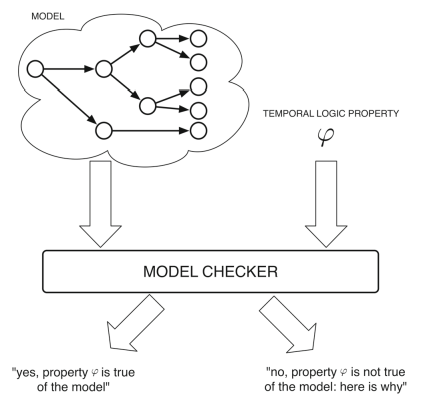
\includegraphics[width=0.75\linewidth]{chapters/checker_over.png}
%    \caption[Model Checking Overview]{Model Checking Overview~\cite{Abate2021}.}
%    \label{fig:modelchecking_flow}
%\end{figure}


%As presented in the picture, one has a set of requirements that need to be satisfied, usually given in a temporal logic (CTL, LTL), stating how the behavior of the systems evolves over time. One also needs to model the system under analysis in such a way that the model checking tool understands it, typically as a Transition System. 

%Once the transition system and temporal logic properties are defined, all that is needed is a model checker to assess whether the specified properties hold within the system.

%There are plenty of model checkers available and, the main difference between them is the algorithm (for optimization purposes). To start this project, some examples of other models Checkers will be described, but the main focus will be on \textbf{Imitator} and \textbf{Uppaal} because, as previously mentioned, it is in these two programs that the systems in Uppex will be shaped. 


\section{Model Checking real-time systems}

Model Checking is an automatic verification technique for finite state (concurrent) systems. Its a very important step in the development of a system to find errors and guarantee correct function \cite{Baier2008}. A summarized picture of the model checking process is given in Figure \ref{fig:modelchecking_flow}.


\begin{figure} [H]
    \centering
    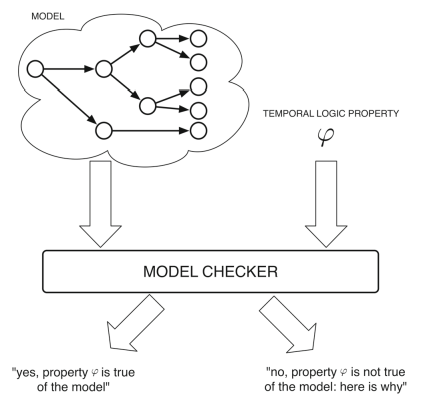
\includegraphics[width=0.75\linewidth]{chapters/checker_over.png}
    \caption[Model Checking Overview]{Model Checking Overview~\cite{Abate2021}.}
    \label{fig:modelchecking_flow}
\end{figure}


As presented in the picture, one has a set of requirements that need to be satisfied, usually given in a temporal logic (CTL, LTL), stating how the behavior of the systems evolves over time. One also needs to model the system under analysis in such a way that the model checking tool understands it, typically as a Transition System. 

%Once the transition system and temporal logic properties are defined, all that is needed is a model checker to assess whether the specified properties hold within the system.

There are many model checkers available, and what mainly distinguishes them is the algorithm they use, since each one adopts different optimization strategies, that is, they all solve the same verification problem but rely on different techniques(add here ref). To start this project, we present different examples of models checkers with\textbf{Imitator} and \textbf{Uppaal} on the spotlight as previously mentioned. It is within these two programs that the systems in Uppex will be modeled and analyzed.

\subsection*{SPIN}

 SPIN is an LTL model checker commonly used for modeling concurrent software and asynchronous processes, particularly communication protocols. It utilizes Promela as the modeling language. After we create our model, it offers the option to simulate the model randomly, interactively, or in a guided manner. Additionally, SPIN can create a C program that automatically performs exhaustive model checking ~\cite{spin}.

%In essence, the process involves the creation of a model system using Promela, which is then subjected to a verification by SPIN. SPIN can either simulate the model through various approaches or generate a C-based verifier. 
The verifier conducts exhaustive model checking, identifying violations of specified properties, such as safety and correctness. This methodology proves particularly valuable in scenarios where correctness and security are critical considerations, as is often the case in communication protocol applications (Figure~\ref{fig:Spin}).

\begin{figure} [H]
    \centering
    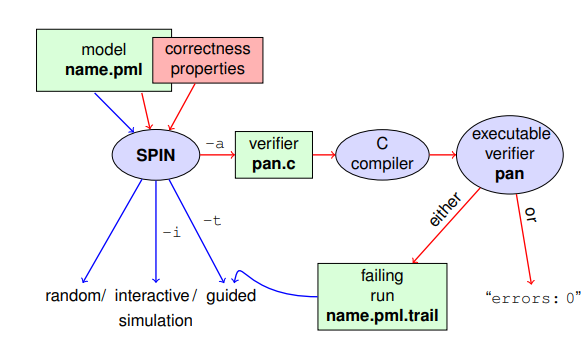
\includegraphics[width=0.75\linewidth]{chapters/spin.png}
    \caption[Spin Process]{Spin Process \cite{spin}.}
    \label{fig:Spin}
\end{figure}

\paragraph{}

\subsection*{Prism}

Prism is a Probabistic Model Checking tool that deals with systems that exhibit probabilistic behavior. Probabilistic model checking refers to a range of techniques for calculating the likelihood of the occurrence of certain events during the execution of systems ~\cite{prism}. As a input, Prism takes a probabilistic model, including \emph{Continuous-time Markov chains} and \emph{Probabilistic timed automata}, and a probabilistic temporal logic \cite{citacao6}. This is summarized in Figure~\ref{fig:prism}.

\begin{figure} [H]
    \centering
    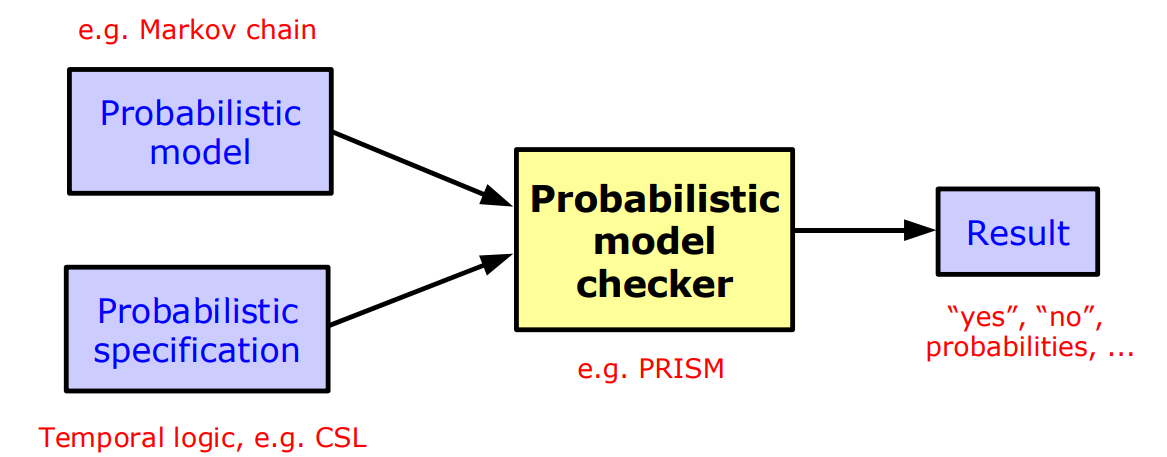
\includegraphics[width=0.9\linewidth]{chapters/Prism.png}
    \caption[Prism Process]{Prism Process~\cite{prism}.}
    \label{fig:prism}
\end{figure}

\paragraph{}

\subsection*{Simulink}

Simulink is a Matlab extension %which is a development and simulation language
that is widely used to \emph{model} and \emph{simulate} dynamical systems~\cite{Peled2001}. It is particularly suitable for specifying mathematical models of real time systems. Simulink has two different approaches to ensure that failures are identified as early as possible.

\begin{itemize}
    \item \textbf{Model testing} attempts to identify failures in models by executing them for some test inputs sampled by a guided randomized algorithm~\cite{Haque2022}.

    \item \textbf{Model checking} attempts to exhaustively verify the correctness of models against some given formal properties~\cite{Haque2022}.
\end{itemize}

In the case of Model checking, the inputs (system and property) are translated and used as inputs in some model checker or Satisfiability Modulo Theories (SMT) solvers. Since Simulink models often represent continuous dynamic and hybrid systems, applying model checking to such models typically leads to undecidable~\cite{Chakraborty2011}.

%colocar o uppaal e imitator

\section{Uppaal in a Nutshell}

As mentioned previously, Uppaal is a model checking tool for verification of real time systems jointly developed by Uppsala University and Aalborg University. In order to do that, Uppaal adopts the concept of Timed (Finite) Automata as model system (transistion system) \cite{Behrmann2006}. 

\subsubsection{Timed Automata}

A \textit{Timed Automaton} (TA) extends the concept of a Finite Automaton with clocks that are used to handle time in the system. Time is continuous and the clocks measure time progress which will increase globally at the same pace for the whole system. It is formally defined as a 6-tuple \cite{baier2008principles}:



\[
\langle L, L_0, Act, C, Tr, Inv \rangle
\]

Where:
\begin{itemize}
    \item \( L \) is the set of \textbf{locations} (or states).
    \item \( L_0 \subseteq L \) is the subset of \textbf{initial locations}.
    \item \( Act \) is the set of \textbf{actions}, and \( C \) is the set of \textbf{clocks}.
    %\item \( Tr \subseteq L \times \mathcal{C} \times Act \times \mathcal{P}(C) \times L \) defines the \textbf{transition relation}, i.e., the rules that determine how the system evolves.
\end{itemize}

Before defining transitions, it is crucial to introduce the concept of a reset. In a timed automaton, the value of a clock can be reset during transitions.

The power set \( P(C) \) represents all possible subsets of the clocks \( C \) that could be reset during a transition ~\cite{baukus2002power}. For example, if \( C = \{x, y\} \), then the power set of \( C \) is:

\[
P(C) = \{\emptyset, \{x\}, \{y\}, \{x, y\}\}
\]

This describes the four possible ways clocks can be reset:

\begin{itemize}
    \item \( \emptyset \): No clocks are reset.
    \item \( \{x\} \): Only clock \( x \) is reset.
    \item \( \{y\} \): Only clock \( y \) is reset.
    \item \( \{x, y\} \): Both clocks \( x \) and \( y \) are reset.
\end{itemize} 

The notation \( \mathcal{C}(C) \) denotes the set of clock constraints over a set \( C \) of clock variables. Each constraint is formed according to \cite{baier2008principles}:

\[
g ::= x \ \square \ n \mid x - y \ \square \ n \mid g \land g \mid \text{true}
\]
where \( x, y \in C \), \( n \in \mathbb{N} \), and \( \square \in \{ <, \leq, >, \geq, = \} \). These will be used in \textbf{guards} (on the transitions) or in \textbf{invariants} (on the locations). It is worth noting that invariants are the only way to enforce a transition \cite{baier2008principles}. 

We can also define the Invariant Function ($Inv$) as follows:

\begin{itemize}
    \item $Inv: L \rightarrow \mathcal{C}(C)$ is the \textbf{invariant function} that assigns a clock constraint to each location $\ell \in L$.
\end{itemize}

With this concepts in place, we can now complete the formal notation for transitions:

\begin{itemize}
    \item \( Tr \subseteq L \times \mathcal{C} \times Act \times \mathcal{P}(C) \times L \) defines the \textbf{transition relation}, i.e., the rules that determine how the system evolves.
\end{itemize}


The transition notation:
\[
\ell_1 \xrightarrow{g, a, U} \ell_2
\]

means that:
\begin{itemize}
    \item The system can transition from location \( \ell_1 \) to \( \ell_2 \) if the \textbf{guard} \( g \) is valid.
    \item The transition is labeled by an \textbf{action} \( a \).
    \item When the transition occurs, the \textbf{clocks} in set \( U \) are reseted.
\end{itemize}

%The power set \( P(C) \) represents all possible subsets of the clocks \( C \) that could be reset during a transition ~\cite{baukus2002power}. For example, if \( C = \{x, y\} \), then the power set of \( C \) is:

%\[
%P(C) = \{\emptyset, \{x\}, \{y\}, \{x, y\}\}
%\]

%This describes the four possible ways clocks can be reset:

%\begin{itemize}
%    \item \( \emptyset \): No clocks are reset.
%    \item \( \{x\} \): Only clock \( x \) is reset.
%    \item \( \{y\} \): Only clock \( y \) is reset.
%    \item \( \{x, y\} \): Both clocks \( x \) and \( y \) are reset.
%\end{itemize} 

%The notation \( \mathcal{C}(C) \) denotes the set of clock constraints over a set \( C \) of clock variables. Each constraint is formed according to \cite{baier2008principles}:

%\[
%g ::= x \ \square \ n \mid x - y \ \square \ n \mid g \land g \mid \text{true}
%\]
%where \( x, y \in C \), \( n \in \mathbb{N} \), and \( \square \in \{ <, \leq, >, \geq, = \} \). These will be used in \textbf{guards} (on the transitions) or in \textbf{invariants} (on the locations). It is worth noting that invariants are the only way to enforce a transition \cite{baier2008principles}. 


Timed Labelled Transition Systems (TLTS) models the execution of TA through labeled transition systems, incorporating so-called delay transitions to capture the passage of time.


A TLTS is a model that introduces two types of transitions \cite{baier2008principles}: 

\begin{itemize}
    \item \textbf{Ordinary transitions}: Associated with actions, denoted by:
    \[
        s \xrightarrow{a} s' \quad \text{where} \quad a \in \text{Act}.
    \]
    \item \textbf{Delay transitions}: Represent the passage of time, denoted by:
    \[
        s \xrightarrow{d} s' \quad \text{where} \quad d \in \mathbb{R}^+_0.
    \]
\end{itemize}

These transitions must obey certain constraints \cite{baier2008principles}:

\begin{itemize}
    \item \textbf{Time additivity}: If \( s \xrightarrow{d} s' \) and \( 0 \leq d' \leq d \), then there exist intermediate states \( s'' \) such that:
    \[
        s \xrightarrow{d'} s'' \xrightarrow{d - d'} s'.
    \]
    \item \textbf{Determinism of delays}: If \( s \xrightarrow{d} s' \) and \( s \xrightarrow{d} s'' \), then necessarily \( s' = s'' \).
\end{itemize}

In terms of semantics, each TA defines a TLTS \( T(TA) \) whose states are pairs of the form \cite{baier2008principles}:
\[
    \langle \text{location}, \text{clock valuation} \rangle.
\]

Transitions follow specific rules, and if a transition depends on a clock \( x \), it only occurs if the associated time constraint is valid. Time can advance as long as the current state still satisfies its constraints.

Clocks are valuation functions \( \eta: C \to \mathbb{R}^+_0 \), mapping each clock \( x \) to its current value. The main operations on clocks are \cite{baier2008principles}:

\begin{itemize}
    \item \textbf{Delay}: Increases the value of all clocks, defined by:
    \[
        (\eta + d)(x) = \eta(x) + d.
    \]
    \item \textbf{Reset}: Resets certain clocks, defined by:
    \[
        \eta[R](x) = 
        \begin{cases}
            0, & \text{if } x \in R, \\
            \eta(x), & \text{otherwise}.
        \end{cases}
    \]
\end{itemize}

More specifically the conversion of a Timed Automaton to a TLTS \( T(ta) = \langle S, S_0, N, T \rangle \) occurs as follows \cite{baier2008principles}:

\begin{itemize}
    \item \( S \) is the set of states;
    \item \( S_0 \) is the set of initial states;
    \item \( N \) is the set of transition labels, including actions and delays;
    \item \( T \) is the set of transitions, defined by:
    \[
        \langle l, \eta \rangle \xrightarrow{a} \langle l', \eta' \rangle \quad \text{if there is a valid transition in } Tr.
    \]
    The delay transition occurs as long as the state invariants are maintained.
\end{itemize}




\subsubsection*{Modelling in Uppaal}

%A system in Uppaal is modeled as a network of TA in parallel \cite{proenca-spreadsheet-2023}. Each automaton is composed by a set of a locations, transistions are used to 'travel' throw all locations and to control those it is possible to use guards, invariant and a synchronization, as we saw before

A system in Uppaal is formally modeled as a network of Timed Automata (TA) that operate in parallel through a composition approach \cite{proenca-spreadsheet-2023}. This network consists of multiple interacting TA processes, where each automaton contains locations (discrete states) and transitions that enable movement between these locations. The behavior is controlled through clock constraints expressed as guards on transitions and invariants on locations, which enforce timing requirements. Additionally, synchronization between different automata is achieved through complementary actions, allowing coordinated behavior across the parallel components \cite{Behrmann2006}. During a Transistion we can also update the value of a variable or clock a \cite{upp}.

%\begin{itemize}
%    \item \textbf{Guard} A guard is a condition applied to the variables and the clocks. If is the condition is True the transistion is enable, otherwise cannot occur~\cite{Behrmann2006}.

%    \item \textbf{Invariants} Invariants are conditions that must be True while the automaton is in a specific location~\cite{Behrmann2006}.

%    \item \textbf{Synchronization}  In Uppaal, synchronization is based on a handshaking mechanism. When two processes take a transition simultaneously, one transition is labeled with \texttt{a!} (send) and the other with \texttt{a?} (receive). In this setup, the exclamation mark ``\texttt{!}'' denotes the sending action that actively triggers the synchronization, while the question mark ``\texttt{?}'' represents the receiving action, which waits for the corresponding send event to occur.

%~\cite{Behrmann2006}.
%\end{itemize}

%During a Transistion we can also update the value of a variable or clock a \cite{upp}.
\paragraph{}

It is now possible to build a model using Uppaal. As an example, it will be built a Worker and Hammer system (\ref{fig:worker model}), as mentioned before.

\begin{figure} [H]
    \centering
    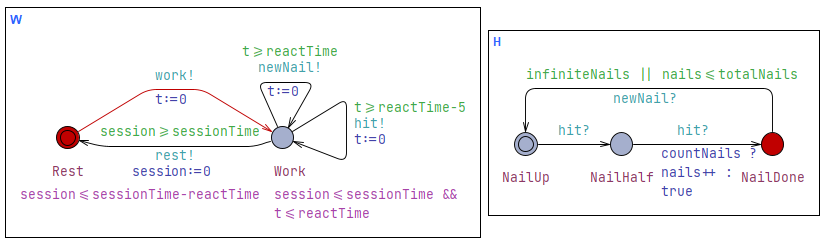
\includegraphics[width=\linewidth]{chapters/worker_hammer.png}
    \caption{Worker/Hammer Automata Example. The image on the left automaton represents the Worker, while the on on the right represents the Hammer.}
    \label{fig:worker model}
\end{figure}

%The worker automaton is made of two states as we see in Figure \ref{fig:worker model}: Rest (initial state) and Work. If the invariant condition is satisfied, a transistion to Work state is taken, synchronized with the event 'press!' and the clock t is restarted. 

%In state Work there are 3 possible transitions but one is excluded while the invariant of that state is satisfied. If t > reactTime,  newNail is done and the clock t is restarted. If t >reactTime -5 the synchronization hit is done and the hammer automata can finally start. When the invariant is no longer satisfied and the system satisfies the guard of the last transition, the automata goes back to the initial state, the clock session is restarted and the process can restart again.

%In Figure \ref{fig:worker model}, the right automaton, as mentioned, represents the Hammer. It has 3 states, none of which have invariants. The first transition occurs only when the "hit" synchronization is activated. The transition from "NailHalf" to "NailDone" happens after the "hit" is activated again, and during this process, the variable "countNails" is updated to a specific value. The last transition back to the initial state is only possible if the logical result of the conditions remains the same, and if the "newNail" synchronization is activated.

%To ensure the model's full functionality, it is essential to declare the variables used in the Uppaal model. The syntax used for declarations is very similar to the one used in C and can be defined as global or local.

%Its important to notice that sessionTime, ReactionTime, totalNails, TotalNail and CountNails are constants and not parameters. Uppaal can not support parameters in clocks, only in variables, if the user pretends to build a generic Process(Timed Automata). In this example sessionTime takes the value 100, ReactionTime 20, totalNails 10 and countNails and infineNails both True.

The Worker automaton consists of two states, as shown in Figure \ref{fig:worker model}: Rest (the initial state) and Work. When the invariant condition is satisfied, a transition to the Work state is triggered, synchronized with the event press!, and the clock t is reset.

In the Work state, there are three possible transitions, although one remains excluded as long as the state invariant holds. If t > reactTime, the transition newNail is executed and the clock t is restarted. If t > reactTime – 5, the synchronization hit is performed, enabling the Hammer automaton to start its execution. When the invariant of the state is no longer satisfied, and the guard of the final transition is met, the automaton returns to the initial state, the session clock is reset, and the process begins again.

In Figure \ref{fig:worker model}, the automaton on the right represents the Hammer. It is composed of three states, none of which contain invariants. The first transition occurs only when the hit synchronization is activated. The transition from NailHalf to NailDone takes place after a second activation of hit, during which the variable countNails is updated to a predefined value. The final transition, which returns the automaton to its initial state, is possible only if the logical conditions remain valid and the newNail synchronization is activated.

To ensure the complete functionality of the model, it is essential to declare the variables used in the Uppaal specification. The syntax for these declarations is very similar to that of C, and variables may be defined as either global or local.

It is important to note that sessionTime, reactionTime, totalNails, totalNail, and countNails are constants, not parameters. Uppaal does not support parameters in clocks, only in variables, when defining a generic process (Timed Automata). In this example, sessionTime is set to 100, reactionTime to 20, totalNails to 10, and both countNails and infiniteNails are set to True.


\subsubsection*{Verification in Uppaal}

The next phase is to check that the model verifies the properties and to do so, Uppaal also has a window dedicated to that (verification window). With Uppaal query language it can be specified the following properties (mentioned above):

\begin{itemize}
    \item \textbf{Reachability properties:} A specific condition that holds in some state of the model’s potential behaviours.

    \item \textbf{Safety properties:} A specific condition that holds in all the states of an execution path.

    \item \textbf{Liveness properties:} A specific condition is guaranteed to hold eventually.

    %\item \textbf{Deadlock properties:} A deadlock is possible or not in the model.
\end{itemize}

These properties can be described using a simple CTL logic variation (TCTL)\cite{lee2009timed}. It is a branching-time temporal logic used to formally specify and verify properties of systems, and it is based on the idea that all possible execution paths a system can take can be represented in the form of a "Computation Tree" \cite{lee2009timed}. The formulas should be one of the following \cite{bengtsson2004timed}:

\begin{itemize}
    \item A[] $\phi$ — Invariantly $\phi$

    \item E<> $\phi$ - Possibly $\phi$

    \item A<> $\phi$ - Always Eventually $\phi$

    \item E[] $\phi$ - Potentially Always $\phi$

    \item $\phi$ $\longrightarrow$ $\psi$ - $\phi$ leads to $\psi$
    
\end{itemize}

The symbols $\phi$ and $\psi$ are formulae that describe state properties, such as what is the current state and clock constrains. Returning to the worker and hammer example, we can illustrate some properties using this notation. Notice that Deadlock is expressed using a special formula and IT consists of the keyword deadlock. 

\begin{itemize}
    \item \textbf{A[]!deadlock} Deadlock never occurs.

    \item \textbf{A[] W.Rest} The Worker always reaches the Rest state.

    \item \textbf{E<> H.NailDone} The Hammer will eventually finish Nailing.

    \item  \textbf{A<> H.NailDone} The Hammer eventually reaches the NailDone state on all paths.

    \item \textbf{W.Work $\longrightarrow$ W.Rest} If the Worker is in the Work state, then it will eventually reach the Rest state.
\end{itemize}

%These properties can be verified on the Verifier, if the property is marked in red it means 'not satisfied' otherwise its satisfied.
These properties can be verified in the Verifier. The Verifier is a tool that checks if your model behaves as expected. If the property is marked in red, it means 'not satisfied' (the model does not guarantee the property). Otherwise, it is 'satisfied' (the model always meets the condition).

%\paragraph{}


%\textbf{Limitations}

%Uppaal is known for its intuitive nature and for being easy to lear, making it accessible even to users with limited knowledge of finite automata. It has a user-friendly interface which facilitates the process of building models, allowing users to create and manipulate designs in a easy way.

%Although its advantages, it has some limitations. For example:

%Uppaal may face limitations when it comes to describing true real-time systems, especially within the context of embedded systems. In many cases, real-time systems are components of larger embedded systems, and the values they receive from the overall system can be predetermined or pre-established.
%One of the challenges with Uppaal is its inability to fully support parameterized clocks and dynamic conditions that may be prevalent in complex real-time systems. Real-time systems often involve intricate interactions with external components, which may have varying inputs and conditions. Uppaal's current capabilities may not fully capture the dynamic and parameterized nature of these interactions, potentially limiting its effectiveness in modeling certain aspects of real-time embedded systems.
%Therefore, while Uppaal may be suitable for certain types of real-time systems, it may not provide the flexibility and expressiveness needed for more intricate embedded systems with dynamic conditions and parameterized clocks. Users may need to consider alternative tools or approaches that better accommodate the complexities of their specific real-time embedded systems.


\section{Imitator in a Nutshell}

IMITATOR is command-line only tool to perform automated parameter synthesis for parameter timed systems. This model checker takes as input a network of Parametric Timed Automata. This type is a sub category of timed automata where clocks can be declared as parameters (without a constant pre-determined), making it particularly useful for modeling \textbf{Real-Time Systems} and \textbf{Software Product Lines (SPLs)}~\cite{IMITATOR}. In real-time systems, timing constraints often depend on environmental conditions or system configurations. By allowing certain timing constraints to remain as parameters rather than fixed values, Parametric Timed Automata enable the analysis of multiple scenarios, ensuring that the system behaves correctly under various conditions \cite{RealTimeSystems}.
Similarly, in Software Product Lines (SPLs), where models need to be adapted and reused across different products or configurations, the use of parametric timing constraints avoids the need to create separate automata for each variation. A single model can be created where critical variables can be written as paramaters. This enhances flexibility and reduces redundancy in system modeling ~\cite{SPL}.


Imitator is a model checker specialized in analyzing parametric systems. Its strength lies not only in verifying whether system properties hold but also in determining the exact conditions (parameter constraints) under which they are satisfied. By using Imitator, we can systematically evaluate a model and check if the properties defined in the property.imiprop file are valid, while also obtaining the precise parameter values required for them to hold. Moreover, Imitator goes beyond mere verification by offering insights into the constraints under which these properties are valid. This information is valuable for understanding the system's behavior and can guide further refinement or optimization to enhance the system's reliability and performance~\cite{IMITATOR}.

\subsubsection{Parametric Timed Automata}

A \textit{Parametric Timed Automaton} (PTA) is a generalization of TA that introduces parameters in the guards and resets of clocks, allowing the modeling of systems where certain temporal values are unknown or variable. Unlike TA, where timing bounds are fixed, PTA enable symbolic analysis and the synthesis of constraints on these parameters. It is formally defined as a 7-tuple \cite{andrePTA}.



\[
\langle L, L_0, Act, C, Tr, \textcolor{red}{P}, Inv\rangle
\]

Where:
\begin{itemize}
    \item \( L \) is the set of \textbf{locations} (or states).
    \item \( L_0 \subseteq L \) is the subset of \textbf{initial locations}.
    \item \( Act \) is the set of \textbf{actions}, and \( C \) is the set of \textbf{clocks}.
    \item \textcolor{red}{\( P \text{ is a finite set of parameters.} \)}
    \item \( Tr \subseteq L \times \mathcal{C}(C) \times Act \times \mathcal{P}(C) \times L \) defines the \textbf{transition relation}, i.e., the rules that determine how the system evolves.
\end{itemize}

The transition notation:

\[
\ell_1 \xrightarrow{g, a, U} \ell_2
\]

Means that:
\begin{itemize}
    \item The system can transition from location \( \ell_1 \) to \( \ell_2 \).
    \item This transition occurs if the \textbf{guard} \( g \) is valid.
    \item The transition is labeled by an \textbf{action} \( a \).
    \item When the transition occurs, the set of \textbf{clocks} \( U \) is reset.
\end{itemize}

The power set \( P(C) \) represents all possible subsets of the clocks \( C \) that could be reset during a transition ~\cite{baukus2002power}. For example, if \( C = \{x, y\} \), then the power set of \( C \) is:

\[
P(C) = \{\emptyset, \{x\}, \{y\}, \{x, y\}\}
\]

This describes the four possible ways clocks can be reset:

\begin{itemize}
    \item \( \emptyset \): No clocks are reset.
    \item \( \{x\} \): Only clock \( x \) is reset.
    \item \( \{y\} \): Only clock \( y \) is reset.
    \item \( \{x, y\} \): Both clocks \( x \) and \( y \) are reset.
\end{itemize} 

The notation \( \mathcal{C}(C) \) denotes the set of clock constraints over a set \( C \) of clock variables. Each constraint is formed according to:

\[
g ::= x \ \square \ n \mid x - y \ \square \ n \mid g \land g \mid \text{true}
\]
where \( x, y \in C \), \( n \in \mathbb{N} \), and \( \square \in \{ <, \leq, >, \geq, = \} \). These will be used in \textbf{guards} (on the transitions) or in \textbf{invariants} (on the locations). It is worth noting that invariants are the only way to enforce a transition \cite{proenca_slides}.

Regarding the semantics of the automaton, we define a \emph{parameter valuation} $v$ as a function that assigns concrete (numerical) values to the parameters $p_1, p_2, \ldots, p_n$ in the automaton. The result of applying $v$ to a parametric timed automaton (PTA) $A$ is denoted by $v(A)$, which corresponds to a non-parametric timed automaton --- that is, all parameters are replaced with specific constant values.

Given a PTA $A = (\Sigma, L, l_0, X, P, I, E)$ and a parameter valuation $v$, the \emph{concrete semantics} of $v(A)$ is defined by a \emph{timed labelled transition system}, as in the case of TA.


A TLTS (Timed Labelled Transition System) introduces two types of transitions:

\begin{itemize}
    \item \textbf{Ordinary transitions}: Associated with actions, denoted by:
    \[
        s \xrightarrow{a} s' \quad \text{where} \quad a \in \text{Act}.
    \]
    \item \textbf{Delay transitions}: Represent the passage of time, denoted by:
    \[
        s \xrightarrow{d} s' \quad \text{where} \quad d \in \mathbb{R}^+_0.
    \]
\end{itemize}

These transitions must obey certain constraints:

\begin{itemize}
    \item \textbf{Time additivity}: If \( s \xrightarrow{d} s' \) and \( 0 \leq d' \leq d \), then there exist intermediate states \( s'' \) such that:
    \[
        s \xrightarrow{d'} s'' \xrightarrow{d - d'} s'.
    \]
    \item \textbf{Determinism of delays}: If \( s \xrightarrow{d} s' \) and \( s \xrightarrow{d} s'' \), then necessarily \( s' = s'' \).
\end{itemize}

In terms of semantics, each Timed Automaton (TA) defines a TLTS \( T(ta) \) whose states are pairs of the form:
\[
    \langle \text{location}, \text{clock valuation} \rangle.
\]

Transitions follow specific rules, and if a transition depends on a clock \( x \), it only occurs if the associated time constraint is valid. Time can advance as long as the current state still satisfies its constraints.

Clocks are valuation functions \( \eta: C \to \mathbb{R}^+_0 \), mapping each clock \( x \) to its current value. The main operations on clocks are:

\begin{itemize}
    \item \textbf{Delay}: Increases the value of all clocks, defined by:
    \[
        (\eta + d)(x) = \eta(x) + d.
    \]
    \item \textbf{Reset}: Resets certain clocks, defined by:
    \[
        \eta[R](x) = 
        \begin{cases}
            0, & \text{if } x \in R, \\
            \eta(x), & \text{otherwise}.
        \end{cases}
    \]
\end{itemize}

The conversion of a Timed Automaton (TA) to a TLTS \( T(ta) = \langle S, S_0, N, T \rangle \) occurs as follows:

\begin{itemize}
    \item \( S \) is the set of states;
    \item \( S_0 \) is the set of initial states;
    \item \( N \) is the set of transition labels, including actions and delays;
    \item \( T \) is the set of transitions, defined by:
    \[
        \langle l, \eta \rangle \xrightarrow{a} \langle l', \eta' \rangle \quad \text{if there is a valid transition in } Tr.
    \]
    The delay transition occurs as long as the state constraints are maintained.
\end{itemize}




\subsubsection{Limitations in Parametric Timed Automata}

Introducing parameters in real-time temporal logic can indeed lead to undecidability issues, notably when such parameters are unbounded. On top of this, the use of multi-rate automata together with linear constraints on clocks also leads to undecidability, as does the use of stopwatches \cite{Andre2021}. The addition of parameters, increases the complexity of the model checking of these systems, this complexity often results in undecidability, meaning that there is no general algorithm that can determine the validity of formulas within the logic. In fact, most interesting problems that are decidable in timed automata become undecidable in Parametric Timed Automata, including the ones below \cite{Andre2021}.


\begin{itemize}
    \item \textbf{EF-emptiness}

    Is the set of parameter valuations for which a given location \( l \) is reachable empty?

    %\textcolor{red}{undecidable}

    \item \textbf{EF-universitily}

    Do all parameters allow to reach a given location \( l \)?

    %\textcolor{red}{undecidable}

    \item \textbf{AF-emptiness}

    Is the set of parameter valuations for which all runs eventually reach a given location \( l \) empty?

    %\textcolor{red}{undecidable}

    \item \textbf{AF-universitily}

    Do all parameters allow to reach a given location \( l \) for all runs?

    %\textcolor{red}{undecidable}

    \item \textbf{Language and Trace Preservation}

    For a given set of timing parameters, are there other parameter values that yield the same sequence of discrete events?

    %\textcolor{red}{undecidable}
\end{itemize}
 

However, there are adaptations that can be applied to the automaton to ensure the decidability of certain problems. For example, reducing parameters, parametric clocks, and non-parametric clocks result in the decidability of the EF-emptiness problem(Parametric clocks are time variables in parametric timed automata whose behavior depends on parameters that are unknown or undefined a priori) \cite{andre2019whats}. Another approach is through the restriction of parameter usage, utilizing a subcategory of Parametric Timed Automata called Lower/Upper Bound Parametric Timed Automata (L/U PTA), where all parameters are compared with the clocks either as an upper bound or a lower bound. With this restriction, several verification problems that are generally undecidable for general PTA become decidable \cite{andre2019whats}. In particular, the EF-emptiness problem (determining whether there exists an instantiation of parameters such that a given state is reachable), the EF-universality problem (checking whether all possible parameter valuations allow the reachability of a given state), and the EF-finiteness problem (determining whether the number of parameter valuations leading to reachability is finite) become decidable. These problems, which are crucial for analyzing the behavior of parametric timed systems, fall within PSPACE complexity when restricted to L/U PTA, ensuring their computational feasibility \cite{andre2019whats}. However, not all verification problems benefit from this restriction. Certain problems remain undecidable even under general PTA constraints. For instance, the AF-emptiness problem (determining whether there exists a parameter valuation such that all runs eventually reach a given state) is undecidable. Similarly, language preservation, which checks whether the language of a PTA remains unchanged under all possible parameter valuations, is also undecidable. Additionally, the EG-emptiness problem (verifying whether there exists a parameter valuation such that some execution remains within a given set of states indefinitely) remains an open question \cite{andre2019whats}.


%Despite these undecidability results, the L/U PTA framework plays a crucial role in retaining decidability for many verification problems, providing a balance between expressiveness and computational feasibility. By ensuring that fundamental reachability and verification tasks remain within PSPACE complexity, L/U PTA continues to be a valuable tool for analyzing real-time systems in fields such as embedded systems, network protocols, and real-time control applications.


%\subsubsection*{Modelling in Imitator}

%The Imitator tool follows the same syntax logic as HyTech and can always be divided into three main parts.

%\begin{itemize}
%    \item \textbf{Variable declarations}

%    In the variable declaration block, we define the essential elements of the model, including constants, parameters, clocks, and state variables. These elements are used to represent temporal constraints and rules within the modeled system.

%    The clocks all evolve at the same rate of 1 time unit, and the way to declare them is with the suffix \textbf{: clocks} after defining their names.

%    Variables can be global or discrete (a name derived from the HYTECH tool syntax). Both are shared by all automata in the model, and unlike discrete variables, the value of global variables cannot be altered. Within discrete variables, there are several types, such as: Integers (Int), Booleans, Arrays, Lists, Stacks, and Queues. Just like with clocks, to declare these variables, you simply use the suffix \textbf{: Type}, where 'Type' represents the desired type from the ones mentioned earlier. 

%    \item \textbf{Automata}

%    In the Automata block, we define the timed automata that represent the system's behavior. It includes states, which represent different phases of the system, and transitions, which define how the system moves from one state to another. Additionally, it contains invariants, which impose constraints on the time that can be spent in a state, guards, which set conditions for a transition to occur, and assignments, which update variables or clocks after a transition.

%    Each location of the automaton is initialized with \textbf{loc}, followed by its name and, if present, an invariant. The definition continues with \textbf{when}, followed by the transition condition, \textbf{sync} for the synchronization action, \textbf{do} for variable or clock updates, and \textbf{goto} to indicate the next state. If there are multiple transitions from the same location, they are listed sequentially.

%    Each location can be urgent if no time passage is allowed in that location, defined by the keyword \textbf{urgent}. This means the system must leave this location immediately without allowing time to elapse. A location can be accepting if it represents a significant final state for verifying liveness properties. Accepting locations are used to define states that must be reached repeatedly in infinite executions, making them useful for checking the recurrence of desired behaviors. It is defined by the keyword \textbf{acepting}.
%    Additionally, a location can combine both properties, being both urgent and accepting, ensuring that the system reaches this location without delay and that it is considered for acceptance conditions in liveness verification.

%    It is also worth noting that the keyword \textbf{Stop} allows certain clocks to be interrupted in specific locations, while \textbf{Flow} enables the modification of the clock's evolution rate.

    
%    \item \textbf{Initial state definition}

%    The initial state definition section is split between the discrete initialization and the continuous initialization.
%    The discrete initialization (introduced by the discrete keyword) assigns an initial value to each discrete (global) variable, and sets the initial location for each automaton.
     %The continuous initialization (introduced by the continuous keyword) defines the initial constraints over clocks and parameters (possibly also using discrete variables).
%\end{itemize}

\definecolor{codebg}{rgb}{0.95,0.95,0.95}
\lstdefinestyle{imitator}{
    backgroundcolor=\color{codebg},
    basicstyle=\ttfamily\small,
    keywordstyle=\color{blue}\bfseries,
    commentstyle=\color{gray}\itshape,
    breaklines=true,
    frame=single,
    keepspaces=true,
    tabsize=4,
    showspaces=false,
    showstringspaces=false
}

%\begin{lstlisting}[style=imitator, caption=Variable Declarations Block]
%var
%    session, t
%    : clock;

%(*@Limits*)
%    sessionTime,
%    reactTime
%    : parameter;
%    nails
%    : discrete;
%    totalNails = 20
%    : constant;
%    b = True,
%    : bool;
%\end{lstlisting}


%\paragraph{}

%\begin{lstlisting}[style=imitator, caption=Automaton Worker]
%(*system*)
%automaton Worker

%synclabs: rest, hit, newNail, Work;

%loc Rest: invariant session <= sessionTime - reactTime
%    when True sync Work do {t := 0} goto Work;

%loc Work: invariant session <= sessionTime && t <= reactTime
%    when t >= reactTime sync newNail do {t := 0} goto Work;
%    when t >= reactTime - 5 sync hit do {t := 0} goto Work;
%    when session >= sessionTime sync rest do {session := 0} goto Rest;

%end
%\end{lstlisting}


%\begin{lstlisting}[style=imitator, caption=Automaton Hammer]
%automaton Hammer

%synclabs: hit, newNail;

%loc NailUp: invariant True
%    when True sync hit goto NailHalf;

%loc NailHalf: invariant True
%    when True sync hit do {nails := nails +1} goto NailDone;

%loc NailDone: invariant True
%    when nails <= totalNails sync newNail goto NailUp;

%end
%\end{lstlisting}


%\paragraph{}


%\begin{lstlisting}[style=imitator, caption=Initial state definition]
%(*system_enc*)
%init := 
%    & loc[Worker] = Rest
%    & loc[Hammer] = NailUp
%    & session = 0
%    & t = 0
%(*@limits2*)
%    & nails = 0
%    & sessionTime >= 0
%    & reactTime >= 0
%    & True;
%end
%\end{lstlisting}



%\paragraph{}


%To check if the system is syntactically correct and in the desired format, we save the code in a file with the .imi extension (e.g., system.imi). Then, we execute the following command in the terminal: \texttt{./imitator system.imi [property.imiprop] [-option]}

 

%The system.imi file serves as a model, representing systems such as the Worker and Hammer system. Alongside, the property.imiprop file contains all the properties that we aim to check. The -option in the command line allows to specify the desired output file format, whether it be PNG, Uppaal, or any other preferred format. It's important to note that the parameters enclosed in square brackets [] are optional~\cite{IMITATOR}.

\subsubsection*{Verification in Imitator}

To synthesize the system's parameters that validate the intended property based on the desired properties, Imitator offers two approaches to the parameter synthetise\cite{IMITATOR}:

\begin{itemize}
    \item \textbf{Synthesis (Synth)}

    IMITATOR attempts to synthesize all parameter valuations satisfying the property.

    \item \textbf{Witness}

    IMITATOR attempts to exhibit at least one parameter valuation satisfying the property.It works like syntesis but stops the analysis as soon as one such set is found
    
\end{itemize}

IMITATOR follows the "Best Effort" paradigm, meaning that attempts to synthesize a set of parameter valuations without guaranteeing termination, due to the undecidable nature of most problems in parametric timed automata. To ensure that the computation eventually halts, the tool relies on approximations, which often results in outcomes that are not sound or complete, meaning the results may include some incorrect parameter values (not sound) or miss some valid ones (not complete). The tool classifies its results into three categories and informs the user about them \cite{imitator_slides}.

\begin{itemize}
    \item \textbf{Exact}

    The synthesis found all and only the correct valuations.

    \item \textbf{Over-approximated}

    The set may contain invalid solutions.

    \item \textbf{Under-approximated}

    Some correct solutions may be missing.

    \item \textbf{Possibly invalid}

    There are no guarantees that the solution is correct.


\end{itemize}

In terms of properties, IMITATOR supports a vast number of properties, including reachability (“EF”), safety (“AG not”), liveness, deadlock-freeness and trace preservation (robustness). Additionally, other algorithms will be discussed in the following chapters, such as Minimum-Time Reachability, which aims to synthesize parameter valuations that minimize the time required to reach a given state, and Optimal Parameter Reachability, which determines the minimum or maximum value of a parameter when reaching a specific state \cite{IMITATOR}. A summary of these properties and their corresponding syntax can be found in Table~\ref{tab:imitator-properties}.
%For example, considering the previous case, we can all synthesize parameter valuations for which the state NailDone in the Hammer automaton is reached at least once using the following query:


%\begin{verbatim}
% #synth EF(loc[Hammer] = NailDone)   
%\end{verbatim}


The result is displayed in the terminal as a printout, showing the constraint applied to the parameters if they exist in the model. Otherwise, the output will be "True" or "False." Additionally, the result can be complemented with a graphical visualization, which can be requested at the end of the command using the options parameter as mentioned above. We will see this applied to examples in the next chapter.


\begin{table}[H]
\centering
\caption{Some Properties and their correspondence syntax in IMITATOR \cite{IMITATOR}}
\label{tab:imitator-properties}
\begin{tabular}{|c|c|}
\hline
\textbf{Property} & \textbf{Syntax Examples} \\ \hline
Deadlock Free & property := synth DeadlockFree ; \\ \hline
Safety & property := synth AGnot(State Predicate); \\ \hline
Reachability & property := synth EF(State Predicate); \\ \hline
Optimal parameter reachability & property := synth EFpmin/pmax(State Predicate,Parameter); %\footnote{Parameter that we want to minimize or maximize}
\\ \hline
Liveness & property := synth CycleThrough(State Predicate); \\ \hline
Robustness & property := synth TracePreservation(Parameters); \\ \hline
\end{tabular}
\end{table}

Other interesting properties are:

\begin{itemize}
    \item \textbf{Inverse Method} 

    \item \textbf{Behavioral cartography} 

    \item \textbf{Minimal-time reachability}

    %Lowest parameter constrain in order to reach certain state in the lowest time~\cite{imi}

\end{itemize}

It is important to note that the CycleThrough algorithm does not cover all Liveness properties. It only verifies whether there exists a cycle in the system (infinitely executable) that visits a given location infinitely often—that is, it ensures that a certain state will eventually be visited and will continue to be visited over time. More complex properties, such as verifying that whenever A occurs, eventually B occurs, or that all executions eventually reach a state X, must be verified using a different algorithm written under the observer formalism \cite{IMITATOR}.

An observer is a parametric timed automaton placed in parallel with the system (usually referred to as the Test Automaton) that neither alters nor constrains its behavior, acting instead as a trigger when a given property is violated. This approach allows more complex properties, such as Safety or Liveness, to be reduced to a Reachability property \cite{observers}.


The synthesis process generates a text file containing a detailed description of the system, along with computational information related to the synthesis, including the type of approximation performed. The key result of interest, the parameter constraint, is located in the section marked by \texttt{BEGIN CONSTRAINT} and \texttt{END CONSTRAINT}. An example of this file can be found in \texttt{Appendix B}, with the mentioned section clearly identified.


\section{Uppex in a Nutshell}

Uppex is a tool that facilitates the creation of a family of software product lines using a list of features defined in an Excel spreadsheet~\cite{uppex}. The process begins by defining configurations, where each configuration represents a unique combination of features. Features correspond to system characteristics, such as "slow" or "fast". Not all feature combinations are valid, some may be semantically inconsistent. To prevent such invalid combinations, Uppex uses a separate sheet where features are organized in a tree-like structure. In this structure, features located on the same leaf cannot be selected simultaneously, ensuring that only meaningful configurations are generated. Additionally, a Limits and Queries sheet is maintained, in which queries are defined through formulas and constants are assigned predefined values according to the configuration being executed. To execute, it is necessary to ensure that both the JVM and Uppaal are installed. Once verified, the latest .jar file can be used to run the command uppex runAll model.xml.

\subsection*{Overview of Software product lines}

We can define a
A software product line (SPL) %as a set of methods used to create similar/generic systems, called variants, from a set of systems that share a set of Features~\cite{Pohl2018}.%\cite{spl,spl2}.
as a technique to describe and develop a family of software products with many common artefacts, which are called \emph{features}. 
Each valid combination of features describes a possible software product from this SPL.
This techniques have been used by many companies, facilitating the development, analysis, and deployment of several large software artefacts with commonalities~\cite{Pohl2018}.
% With this, companies that implement the systems save time and money in production and focus on other developments~\cite{Pohl2018}.
%
There are many ways to implement SPL, which can be grouped %most of them
into two groups~\cite{Pohl2018}:

\begin{itemize}
    \item \textbf{Compositional Approaches}
    \item \textbf{Annotative Approaches}
\end{itemize}

In Compositional Approaches, features are treated as separate systems or code fragments that extend the base code. The key idea is to compose them in parallel. After defining certain features, they are integrated into the system. This integration can be done in different ways, ranging from simple concatenation to complex code transformations. Among the various types of parallel composition, the most notable are: \textbf{feature-oriented programming}, \textbf{aspect-oriented programming}, and \textbf{delta-oriented programming}.

In the other hand we have Annotative Approaches where annotations or markings are used to control the presence or absence of the Features that we want to add to the system (in this case they are already present in the base code). For example, in C and C++ programming languages, preprocessor directives such as ifdef, ifndef, else, and endif are used to conditionally include or exclude blocks of code during compilation.


\subsection*{Overview of Uppex}

Uppex is a tool developed in Scala that uses Apache POI libraries to read Microsoft documents. Its main goal is to simplify the construction and verification of multiple Uppaal models generated from different configurations of a single file, following the principles of Software Product Lines previously studied. The tool relies on an annotation mechanism to allow customization of various parts of the model, such as channels, shared variables, data types, time bounds, and requirements.

Uppex reads an Excel file containing the configurations and a Uppaal file with the source model with annotations, and generates a new Uppaal file for each configuration found. Each generated file replaces the original model and is verified by Uppaal. The output is an HTML report summarizing the generated configurations and the properties that were verified. The workflow follows the structure illustrated in Figure \ref{fig:Uppex WorkFlow}.

\begin{figure} [H]
    \centering
    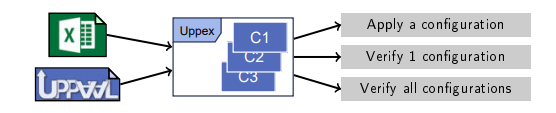
\includegraphics[width=\linewidth]{images/uppex_flow.png}
    \caption{Uppex WorkFlow \cite{proenca_uppex}}
    \label{fig:Uppex WorkFlow}
\end{figure}

The declarations that indicate annotations in the Uppaal file follow the format \textit{"// @Name"} and continue until a blank line is encountered. These serve as hooks that allow Uppex to inject and update the values used to configure the model, and are referred to simply as annotations. To inject and update the queries to be verified for each configuration, a different annotation is used, called a XML annotation. As the name suggests, it encompasses blocks that start with \textit{"<Name>"} and end with \textit{"</Name>"}. Each of these annotations is defined in the Excel file on a sheet with the same name. The first cell of the sheet specifies the pattern to be followed in order to generate the code that will be injected into the annotation block with the corresponding name in the Uppaal file. This is followed by a table where one column contains the name of the variable to be inserted, and the next columns specify the type and value of the variable separately. Additionally, there is a column named Feature that indicates which variables are active in the current configuration, discarding the others. In cases where duplicate variable names exist, only the last occurrence is considered. The configuration declarations are defined in the "@Configurations" sheet, with each configuration representing a combination of the existing features.To control the valid combinations of features, there is another sheet named "@FeatureModel", where the features are organized in a tree structure. In this structure, features that share the same root node cannot be selected simultaneously.

\subsection*{Revisiting the Worker and Hammer example}

%To better understand how it works, we can use the Worker and Hammer system as an example.
We will use the Worker and Hammer system to illustrate our description.


%Model Checking real time systems is a complex task because of nondeterminism and large number of states, which quickly leads to an explosion of states.

%One of the ways to combat this problem is to use the Uppex tool. Its a command only tool with a Excel file as frontend. From a generic model of a system and with Features selected by the user supports the creation and verification of variations of this model. Variations with fewer states and simpler. Another advantage of the tool is that the interaction between the user and the tool is through an excel file which reduces interaction with the Checker model~\cite{uppex,uppex-railway}. The model checker used by Uppex is Uppaal.


\begin{figure} [H]
    \centering
    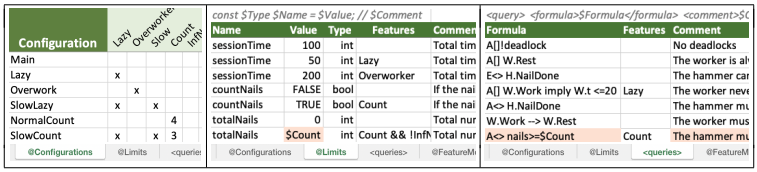
\includegraphics[width=\linewidth]{chapters/uppex.png}
    \caption{Uppex Configuration, Limits and Queries Sheets}
    \label{fig:WH_uppex}
\end{figure}

\begin{figure} [H]
    \centering
    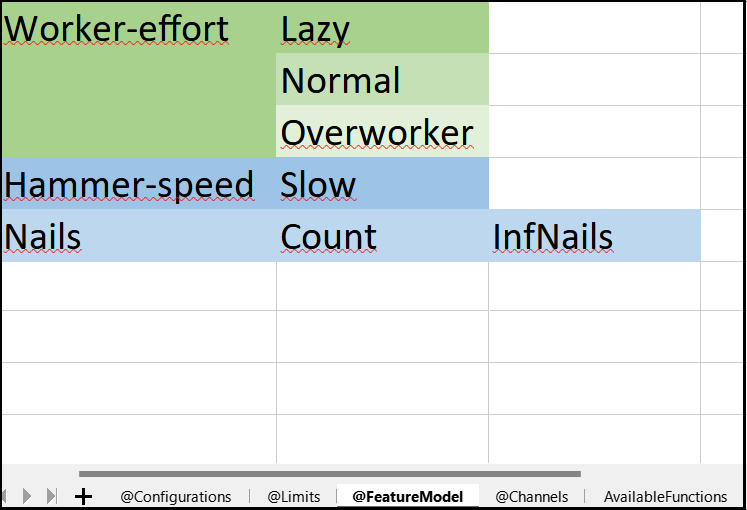
\includegraphics[width=0.4\linewidth]{images/upe_WH.png}
    \caption{Uppex Feature Model Sheet}
    \label{fig:WH_FM}
\end{figure}

Figure \ref{fig:WH_uppex} represents the Configurations, Limits, and Querie sheets, respectively. Assuming Lazy is the active configuration, the annotation block is rewritten using the following pattern:\texttt{const \$Type \$Name = \$Value; //\$Comment}, where the \texttt{\$} notation identifies the column from which the value should be extracted and replaced. Furthermore, as previously explained, only the values whose Feature matches the selected configuration (in this case, Lazy) are left blank will be considered.
\paragraph{}

%% usar fonte do codigo imitator

\begin{figure}[H]
\centering
\begin{minipage}{2.9\linewidth}
\begin{lstlisting}[language=MOREUPPAAL]
// @Limits
const int sessionTime = 50; // Total time that the worker can work
                            // before stopping 
const bool countNails = false; // If the nails should be counted. 
// If so, the system will have an infinite amount of states. 
const int totalNails = 0; // Total number of new nails available
                          // (when counting nails) 
const bool infiniteNails = false; // If there is no bound on the
                          // number of nails (can cause overflows) 
const int reactTime = 20; // Maximum time that the worker can take to
                          // hit or place a new nail 
\end{lstlisting}
\end{minipage}
\caption{Limits Block Rewritten with new values}
\label{fig:worker-config}
\end{figure}

The "<queries>"" sheet follows the same principle, but in this case it corresponds to an XML annotation that defines temporal properties to be verified by UPPAAL. Each query is represented according to the structure:

\texttt{<query><formula>$Formula</formula><comment>$Comment</comment></query>}

Where the \texttt{formula} specifies the property to be checked and the \texttt{comment} provides a human-readable description. An example of a "<queries>"" block is presented below, where different temporal logic properties are expressed to ensure system correctness, such as the absence of deadlocks, the ability of processes to reach certain states, and behavioral constraints between actions:

\begin{figure}[H]
\centering
\begin{minipage}{0.9\linewidth}
{\footnotesize
\begin{verbatim}
<queries>
<query>
<formula>A[]!deadlock</formula>
<comment>No deadlocks</comment>
</query>
<query>
<formula>A[] W.Rest</formula>
<comment>The worker is always resting</comment>
</query>
<query>
<formula>E<> H.NailDone</formula>
<comment>The hammer can finish a nail</comment>
</query>
<query>
<formula>A<> H.NailDone</formula>
<comment>The hammer must complete a nail</comment>
</query>
<query>
<formula>W.Work --> W.Rest</formula>
<comment>The worker must be able to rest after working</comment>
</query>
</queries>
\end{verbatim}
}
\end{minipage}
\caption{Example of a \texttt{<queries>} block specifying temporal logic properties in UPPAAL.}
\end{figure}
\caption{Queries Block Rewritten with new values}
\label{fig:worker-config}
\end{figure}

It is also important to highlight the constraints on feature combinations illustrated in Figure \ref{fig:WH_FM}. For instance, the user cannot select both Lazy and Overworker in the same configuration, thus preventing illogical or inconsistent combinations. Once the Excel configuration is complete, Uppex can be executed. The tool is distributed as a .jar file, which means it can be run directly from the command line. Uppex offers several execution options, allowing for flexible use depending on the user's needs. For example, it is possible to:

\begin{itemize}
    \item Run a specific configuration only (e.g., run the configuration named Main);

    \texttt{java -jar uppex.jar --run -p Main Model.xml}

    \item Validate the model and input files before generating the Uppaal models;
    
    \texttt{java -jar uppex.jar --validate Model.xml}
    
    \item Run all configurations defined in the Excel file, generating one Uppaal model for each and verifying the corresponding properties;
    
    \texttt{java -jar uppex.jar --runAll Model.xml}
\end{itemize}

As an example, we will choose the last option and run all configurations. When executed, Uppex generates an HTML report as output, summarizing the models and properties analyzed for each configuration. For the previous example, the resulting report can be found in the attachment.


%Sheet Configurations is responsible for variations of the Hammer and Worker file in uppaal. If we recall the worker and hammer example in the 'Uppaal in a Nutshell' section we had declared the variables sessionTime,countNails,totalNails,infiniteNails and reactTime and we had given a value to show how the tool works. It turns out that the Uppex tool takes these variables and depending on the settings they receive certain values. For example if we select Lazy, the sessionTime variable takes the value 200. The same happens with queries, are also checked according to the settings of the first sheet~\cite{uppex}.



%\section{The problem and its challenges}

%The next steps will consist of a first phase in the Imitator Connection with the Uppex Tool ensuring that it meets the same features that were already guaranteed by Uppaal. In a second resort take advantage of the capabilities of parameter synthesis (something that as we mentioned is not allowed in Uppaal) and apply these to Uppex.

%The next steps will consist of two main phases aimed at integrating and extending the capabilities of the Uppex tool. In the first phase, the focus will be on establishing a connection between Uppex and Imitator, ensuring that the tool can replicate the same functionalities and behavioral guarantees that were previously achieved through Uppaal. This includes verifying that the model configurations generated by Uppex remain valid and correctly verifiable when passed to Imitator, especially regarding the timing constraints, synchronization channels, and logical properties. The goal is to maintain functional parity with Uppaal while enabling compatibility with Imitator's framework.

%In the second phase, the aim is to leverage Imitator’s powerful capabilities for parameter synthesis—a feature that, as previously discussed, is not supported by Uppaal. By integrating parameter synthesis into the Uppex workflow, it becomes possible to not only verify specific configurations but also explore ranges of parameter values for which certain properties hold. This enhancement would allow the tool to support more advanced forms of design-space exploration, robustness analysis, and automated configuration tuning, significantly expanding the potential use cases of Uppex beyond traditional model checking.

%Ultimately, this extension will enable Uppex to support a broader class of problems and contribute to the development of more flexible and intelligent verification workflows in systems modeled with timed automata.

\section{Proposed extensions to Uppex}

%%colocar as secções deste capitulo

With the Imitator Model Checker and the Uppex tool introduced, the following chapters will detail the integration of Imitator into Uppex's backend as an alternative Model Checker to Uppaal. This integration also brought improvements to the types of supported features, the range of accepted properties and models, as well as enhancements to the final report generated by Uppex. Additionally, the first steps were taken toward developing a graphical user interface for the tool, aiming to provide a more user-friendly experience and reduce reliance on the terminal.



%como e que a nossa contribuição se relaciona com o que ja existe
